\documentclass[10pt,a4paper,fontset=none]{ctexart}

\usepackage[
  top=1.25cm,
  bottom=0.25cm,
  left=0.9cm,
  right=0.9cm
]{geometry}
\usepackage{enumitem}
\usepackage{eso-pic}
\usepackage{fontspec}
\usepackage{graphicx}
\usepackage{pifont}
\usepackage{tabularx}
\usepackage{titlesec}
\usepackage{xcolor}

\setmainfont[BoldFont={Microsoft YaHei Bold}]{Microsoft YaHei}
\setCJKmainfont[BoldFont={Microsoft YaHei Bold}]{Microsoft YaHei}
\setCJKsansfont[BoldFont={Microsoft YaHei Bold}]{Microsoft YaHei}
\CJKsetecglue{}

\pagestyle{empty}
\setlength{\parindent}{0pt}
\setlength{\parskip}{0pt}
\renewcommand{\baselinestretch}{1.5}

\newcommand{\sectionFont}{\fontsize{11pt}{11pt}\selectfont\bfseries}
\newcommand{\entryTitleFont}{\fontsize{10pt}{10.8pt}\selectfont\bfseries}
\newcommand{\bodyFont}{\fontsize{9pt}{10.8pt}\selectfont}
\newcommand{\dateFont}{\fontsize{9pt}{9pt}\selectfont}
\newcommand{\entryIndent}{0.3cm}
\newcommand{\sectionRule}{\vspace{0.1cm}\titlerule[1pt]}

\titleformat{\section}
  {\sectionFont}
  {}
  {0pt}
  {}
  [\sectionRule]
\titlespacing*{\section}{0cm}{0.3cm}{0.3cm}

\setlist[itemize]{
  label=\raisebox{0.75pt}{\fontsize{7.5pt}{7.5pt}\selectfont\ding{108}},
  labelindent=0.3cm,
  leftmargin=*,
  rightmargin=0.3cm,
  labelsep=0.45em,
  itemsep=0pt,
  topsep=0pt,
  parsep=0pt,
  partopsep=0pt
}

\newcommand{\resumeName}[1]{%
  {\centering\fontsize{12pt}{12pt}\selectfont\bfseries #1\par}%
}

\newcommand{\resumeContact}[1]{%
  {\centering\fontsize{10.5pt}{10.5pt}\selectfont #1\par}%
}

\newcommand{\schoolEntry}[3]{%
  \begingroup
  \leftskip=\entryIndent
  \rightskip=\entryIndent
  \parfillskip=0pt
  \entryTitleFont
  \noindent
  \makebox[0pt][l]{#1}\hfil #2\hfil\makebox[0pt][r]{{\dateFont #3}}\par
  \endgroup
}

\newcommand{\twoSideEntry}[2]{%
  \begingroup
  \leftskip=\entryIndent
  \rightskip=\entryIndent
  \entryTitleFont
  \noindent #1\hfill{\dateFont #2}\par
  \endgroup
}

\newenvironment{eduItems}{%
  \begin{itemize}%
}{%
  \end{itemize}%
}

\newenvironment{eduItemsSecond}{%
  \begin{itemize}%
}{%
  \end{itemize}%
}

\newenvironment{resumeItems}{%
  \begin{itemize}%
}{%
  \end{itemize}%
}

\newcommand{\resumeText}[1]{
  {\bodyFont #1}
}
\newcommand{\resumeIntroText}[1]{%
  \begingroup
  \leftskip=\entryIndent
  \rightskip=\entryIndent
  \bodyFont
  \noindent #1\par
  \endgroup
}

\newcommand{\resumeItem}[1]{\item \resumeText{#1}}

\newcommand{\resumePhoto}{
  \AddToShipoutPictureFG*{
    \AtPageUpperLeft{
      \put(494,-84){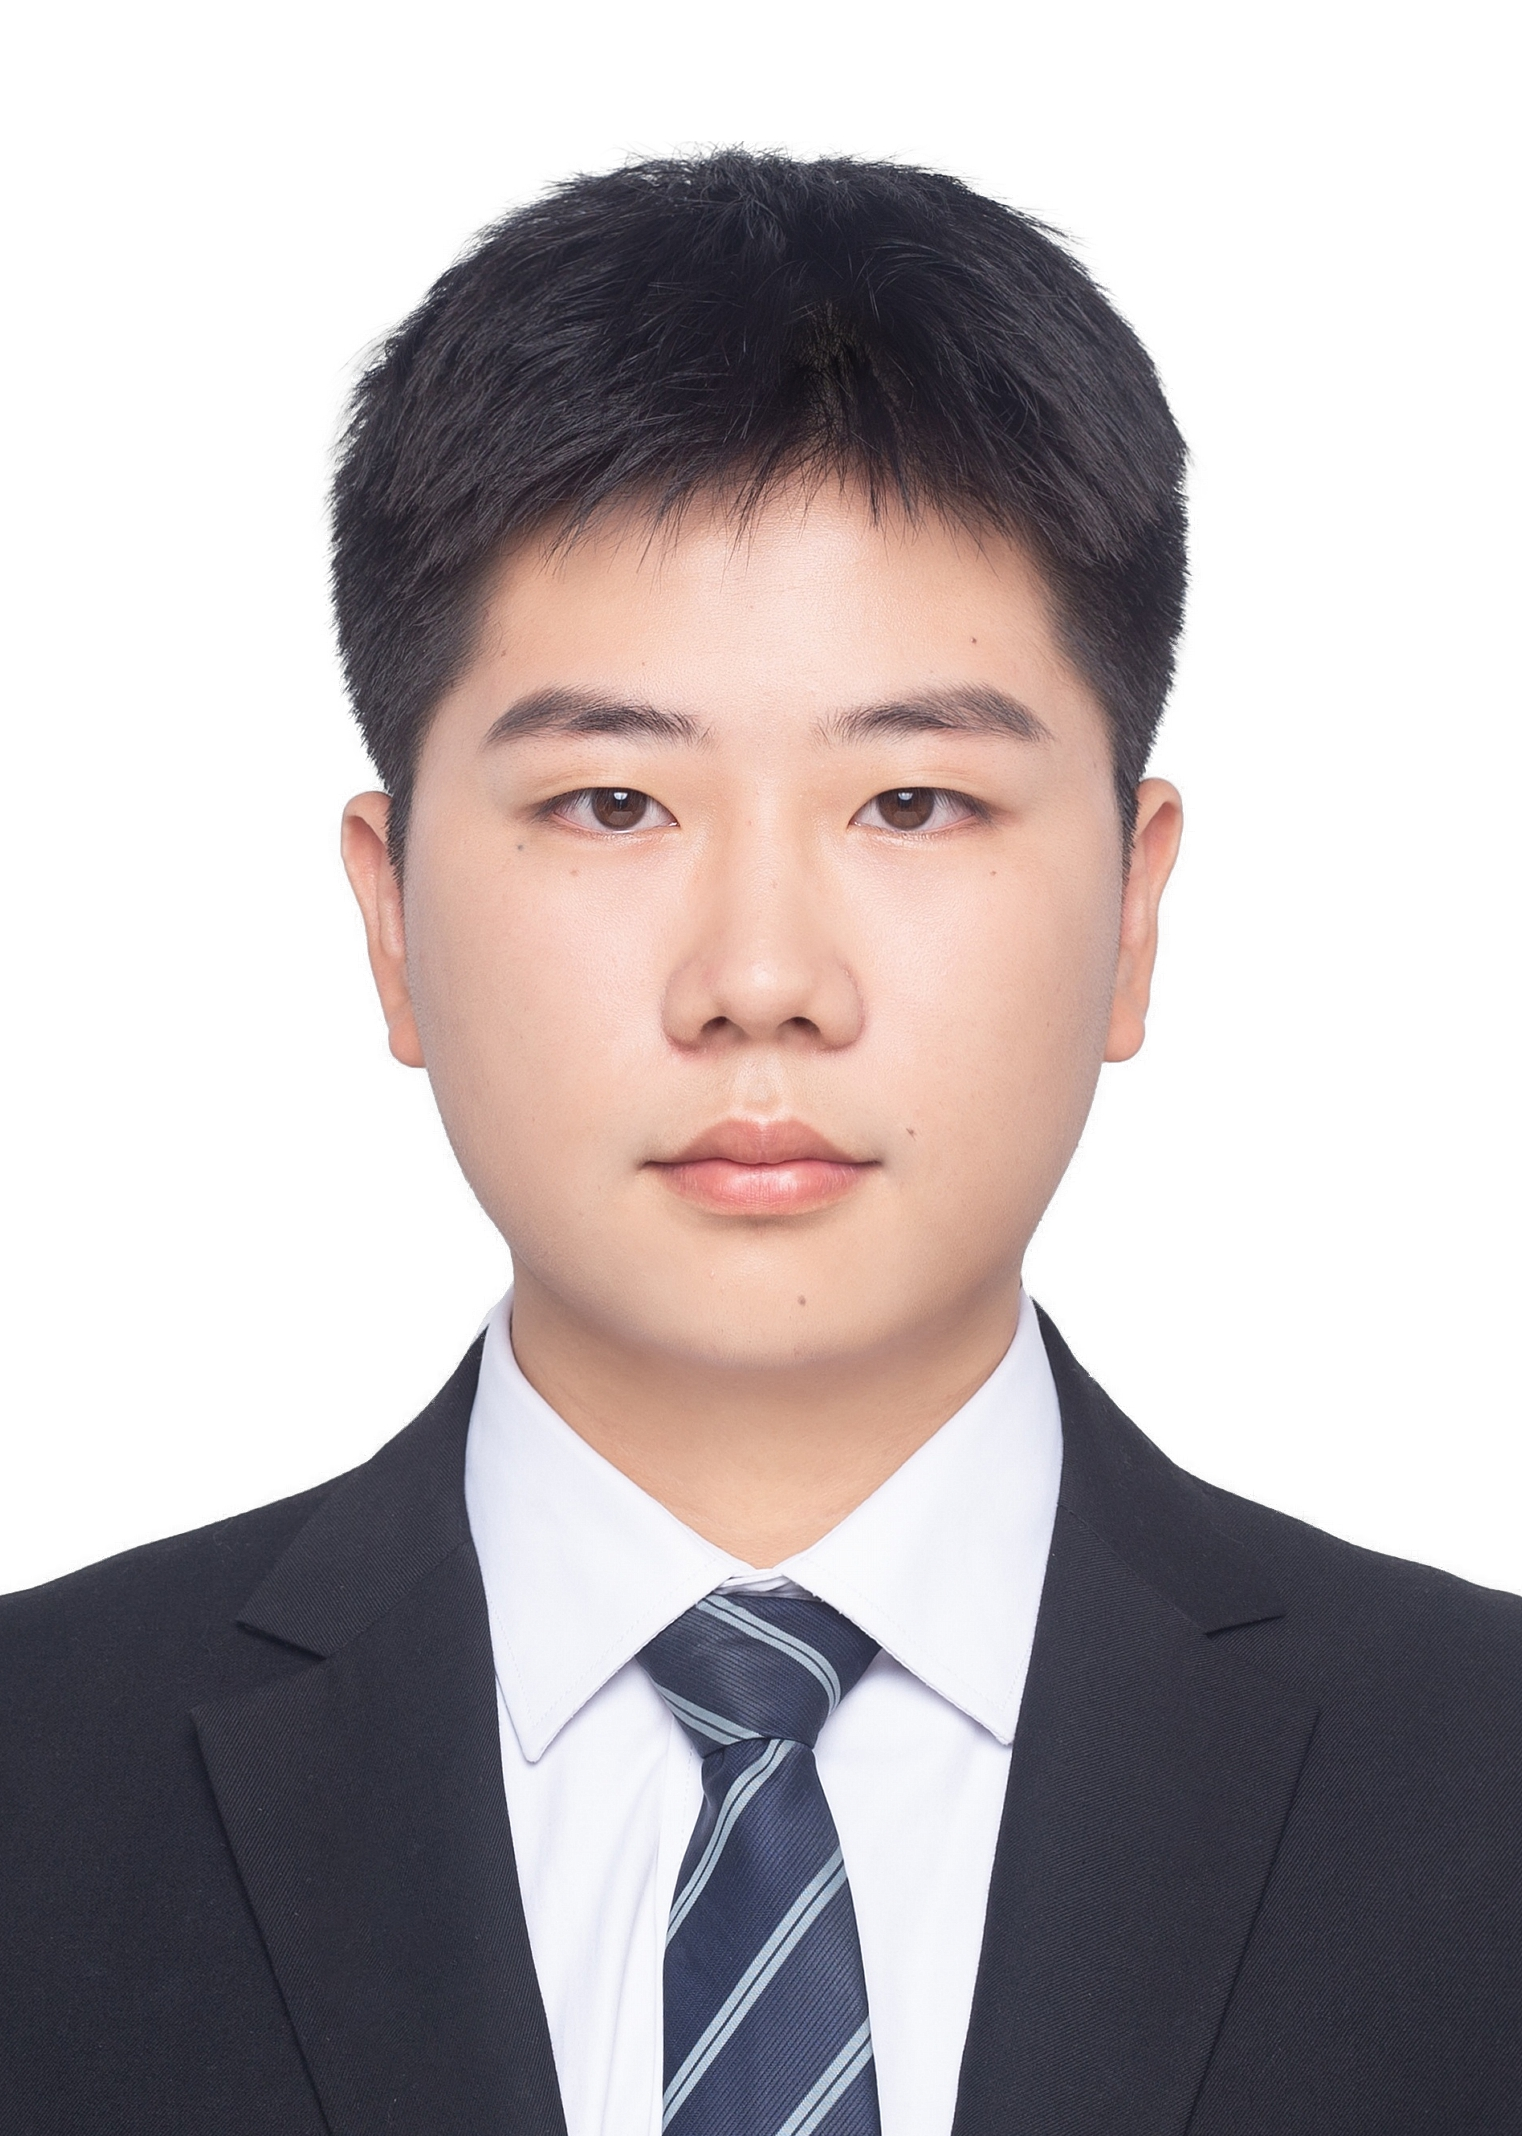
\includegraphics[width=52pt,height=74pt]{id_photo.jpg}}
    }
  }
}

\begin{document}
\bodyFont

\resumePhoto
\resumeName{吴昱}
\vspace{3pt}
\resumeContact{18279277705 \,|\, wyfofo@163.com \,|\, 中共党员}

\section{教育背景}
\schoolEntry{北京交通大学（硕士）}{交通信息工程及控制}{2024年09月 -- 2027年06月}
\begin{eduItems}
  \resumeItem{\textbf{在校经历：} GPA：3.62/4.0（实验室第一）、担任IEEE北京学生分会外联部部长、班级党支部纪检委员、获得一等学业奖学金。}
\end{eduItems}

\schoolEntry{华东交通大学（本科）}{自动化}{2020年09月 -- 2024年06月}
\begin{eduItemsSecond}
  \resumeItem{\textbf{在校经历：} GPA：3.56/4.0（前 5\%）、通过了CET-6、多次获得优秀学生奖学金和优秀学生、获得数模和电赛等市级奖项。}
\end{eduItemsSecond}

\section{实习经历}
\twoSideEntry{字节跳动 -- TikTok Social \,|\, 后端开发实习生}{2025年04月 -- 至今}
\resumeIntroText{\textbf{背景：}TODO}
\begin{resumeItems}
  \resumeItem{\textbf{计算资源优化：}AB 调用进行小包改造并接入 Abase 缓存，降低服务自身 30\% 的计算资源消耗，延迟 -50\%（P99 470ms -> 250ms），US机房稳定性从 99\% 提升至 99.99\%；}
  \resumeItem{\textbf{稳定性报警治理：}核心场景报警覆盖率达到 95\%，周电话报警数量 <50，报警 Mac 化；}
  \resumeItem{\textbf{日志治理：}Comment/Notice 日志降级问题优化，关键日志打标。}
  \resumeItem{\textbf{平台 AI 审批能力迭代：}TODO}
  \resumeItem{\textbf{Oncall Agent 建设：}TODO}
\end{resumeItems}

\twoSideEntry{美团 -- 搜索和推荐平台部 \,|\, AI 应用实习生}{2025年12月 -- 2026年04月}
\resumeIntroText{\textbf{背景：}当前问小团已从单点验证阶段迈入多业务扩张期，面对 15 个业务线的快速接入需求，现有分散式架构导致了系统重复建设、效率参差不齐以及性能缺乏管控等问题，制约了 AI 搜索能力的规模化应用，亟需构建统一的 AI 搜索开放平台。}
\begin{resumeItems}
  \resumeItem{\textbf{AgentEnv 工具环境建设：}负责 Agent 训练所依赖的工具执行环境服务的开发与迭代，支持各种工具的稳定接入；设计并实现削峰队列解决下游工具限流问题，引入空值重试机制提升工具调用稳定性；实现 Caffeine + Cellar 多级缓存，降低训练成本；}
  \resumeItem{\textbf{工具监控与稳定性改造：}设计并落地工具调用全链路监控体系，包含多维度指标，接入 Raptor 告警，实现工具健康状态自动感知；设计 Token 鉴权机制，支持调用来源溯源；通过反射将工具以 HTTP 接口形式暴露出去，解决了 SSE 长连接导致的问题；}
  \resumeItem{\textbf{工具配置化：}将工具接入方式从硬编码重构为动态配置，支持灵活配置工具各项参数，新工具接入无需发布，迭代效率大幅提升；}
  \resumeItem{\textbf{训练样本合成：}独立负责训练样本合成模块的设计与开发，包括库表结构设计、基于 Airflow 的批量数据蒸馏任务调度、S3 文件存储、样本集版本管理与合并等全链路功能，对外提供完整的 RESTful API。}
  \resumeItem{\textbf{并行工具调用器：}基于 CompletableFuture 实现并行工具调用执行器，支持 AI 搜索 Agent 在单次推理中并发调用多个工具，统一等待所有任务完成后汇总结果，相比串行执行工具调用阶段耗时降低。}
\end{resumeItems}

\twoSideEntry{明略科技 - 用户增长部门 \,|\, Java 实习生}{2025年09月 -- 2025年12月}
\resumeIntroText{\textbf{背景：}公司启动“秒知”企业知识库建设，打造基于 RAG 架构的智能知识管理平台，支持多格式文档解析、向量化存储与语义检索能力，构建统一的企业私有知识服务体系，提升内部知识沉淀与复用效率，并为后续业务系统提供可复用的智能问答能力底座。}
\begin{resumeItems}
  \resumeItem{\textbf{权限体系建设：}基于 Spring Security + JWT 实现基于组织标签的 RBAC 的多级权限系统，使用 Redis 管理 Token 的生命周期，通过用户角色、组织归属和文件属性的权限过滤，实现精细化的文档访问控制，确保敏感数据安全；}
  \resumeItem{\textbf{文件上传：}实现大文件分片上传与断点续传机制，使用 Redis 的 Bitmap 记录分片状态，并通过 MinIO 按照 MD5 进行分片合并，基于 Kafka 解耦文件处理流程；}
  \resumeItem{\textbf{知识构建与检索：}将解析后的文档按语义进行分块，将文本内容、向量及权限、标签等元数据同时存入 Elasticsearch，实现混合检索，并对召回片段进行重排与去重后拼接为增强型 Prompt。}
\end{resumeItems}

\section{专业技能}
\begin{resumeItems}
  \resumeItem{熟练掌握 Java 基本语法，深入理解面向对象编程思想，熟悉 Java 内存模型和垃圾回收机制，对数据结构和算法有一定的了解；}
  \resumeItem{熟练使用 MySQL，了解数据库的事务、索引等概念，对 Redis、Elasticsearch 等非关系型数据库有一定的了解和使用经验；}
  \resumeItem{熟练使用 Spring Boot、Spring Cloud 框架，理解 IOC 和 AOP 原理，熟悉 MyBatis 等 ORM 框架，了解微服务架构；}
  \resumeItem{理解线程的概念、生命周期，能等够创建和管理线程，掌握线程同步的方法，了解线程安全问题，熟悉并发容器的使用；}
  \resumeItem{了解操作系统的基本概念，如进程管理、内存管理等，掌握计算机网络基础知识，如 TCP/IP 协议、HTTP 协议等。}
\end{resumeItems}

\end{document}
